\documentclass[../Main.tex]{subfiles}

\begin{document}

\chapter{LES SÉRIES NUMÉRIQUES}

\intro{
\textbf{Prérequis}
\begin{itemize}
    \item Développement limité.
    \item Manipuler les Inégalités.
\end{itemize}

\textbf{Objectifs}
\begin{itemize}
    \item Savoir montrer la convergence/divergence d'une série Numérique.
    \item Savoir utiliser les séries numériques pour étudier les suites.
\end{itemize}
}{
Dans ce chapitre, on acquerra l'un des compétences indispensables pour faire le chapitre d'étude des fonctions définit par série, ce qui est le tiers de programme d'analyse. \\ 
Dans ce chapitre, on prend $(u_n)_{ n \in \NN }$ une suite réelle ou complexe. On appelle somme partielle de $u_n$ la suite $ S_n = \sum_{i=0}^n u_i$, s'elle diverge, on dit que la série de terme générale $u_n$ est divergente et on écrit \diverge, sinon s'elle converge, on dit que la série de terme générale $u_n$ est convergente et on écrit \conv ,et Dans le cas de convergence, on définit la série reste $R_n(u)=\sum_{i=0}^n u_i$. Dans tout chapitre, on verra les méthodes qui vont nous permettent de décider la nature d'une série numérique [conv ou div].
}

\section{Séries Numériques définis explicitement} 
Dans cette section, on verra des théorèmes qui permettent de juger la nature d'une série lorsque qu'on sait une expression explicite de son terme générale. Sinon, on verra dans les sections suivantes une utilisation indirecte de ces théorèmes pour déterminer la nature des séries qui ne sont pas explicitement exprimées.
\subsection{Les théorèmes fondamentaux des séries numériques} 
		\thm{Critère séquentiel des séries alternés \label{thm:CSSA}}{
			On dit que la suite $(u_n)_{ n \in \NN }$ vérifie critère séquentiel des séries alternées [CSSA] lorsqu'elle vérifie :
			\begin{itemize}
				\item $ \forall n \in \NN \two u_n = (-1)^n |u_n| $ 
				\item $ ( |u_n| )_{ n \in \NN } $  est décroissante 
				\item $ u_n \longrightarrow 0$ 
			\end{itemize}
			Et dans ce cas \conv 			}
   
		
		\thm{Règle de D'Alembert \label{thm:Regle D'Alembert}}{
			Si la suite $(u_n)_{ n \in \NN }$ est strictement positive à partir d'un certain rang [APCR] alors : 
		\\ on calcule, si elle existe, $$  l=\lim_{n \to \infty} \frac{u_{n+1}}{u_n} \geq 0 $$ 
		\\ et on discute les cas : 
		\begin{itemize}
			\item Si $ l < 1 $ alors \conv 
			\item Si $ l > 1 $ alors \diverge 
			\item Si $ l = 1 $ On ne peut rien conclure 
		\end{itemize}
		}


		\thm{Règle de Cauchy \label{thm:Règle de Cauchy}}{
			Si la suite $(u_n)_{ n \in \NN }$ est positive [APCR] alors : 
		\\ on calcule, si elle existe, $$  l=\lim_{n \to \infty} \sqrt[n]{u_n} \geq 0 $$  
		\\ et on discute les cas : 
		\begin{itemize}
			\item Si $ l < 1 $ alors \conv 
			\item Si $ l > 1 $ alors \diverge 
			\item Si $ l = 1 $ On ne peut rien conclure 
		\end{itemize}
		}
  
		\thm{Règles de comparaison \label{thm:Régles de comparaison (series)}}{
        Si les deux suites $(u_n)_{ n \in \NN }$ et $(v_n)_{ n \in \NN }$ sont positives [APCR] Alors, on a : 
		\begin{itemize}
			\item $u_n  = o(v_n)$ \ Alors, on a :  $ \sum v_n$ conv $\Rightarrow$ \conv et \diverge $\Rightarrow$ $ \sum v_n$ div  
			\item $ u_n = O(v_n)$ Alors, on a :  $ \sum v_n$ conv $\Rightarrow$ \conv  et \diverge $\Rightarrow$ $ \sum v_n$ div 
			\item $ u_n \leq v_n $   \ \ \ \ \  Alors, on a :  $ \sum v_n$ conv $\Rightarrow$ \conv et \diverge $\Rightarrow$ $ \sum v_n$ div  
			\item $ u_n \sim v_n$ \ \ \ \ \  Alors, on a :  $ \sum v_n$ conv $\Leftrightarrow$ \conv et \diverge $\Leftrightarrow$ $ \sum v_n$ div
		\end{itemize}
}

		\cor{ \label{cor:Serie-Ref} Séries Référentielles :  }{
		Les Règles de comparaison ne sont pas assez utiles si on n'a pas des séries de référence pour comparer avec, c'est le but de ce corollaire : \\
			\textbf{Série géométrique : } \\
			- La suite $(q^n)_{ n \in \NN }$ conv ssi $|q|<1$  \\
			\textbf{Série de Riemann : } \\
			- La suite $\left(\frac{1}{n^\alpha}\right)_{ n \in \NN }$ conv ssi $\alpha>1$
}


		\thm{comparaison avec intégrale}{
			Soit $ f : \RR^+ \longrightarrow \RR^+$ une fonction décroissante et continue sur $\RR^+$.
			\\ Si on suppose que : $\forall n\in\NN \two u_n=f(n)$ alors : 
			\\ les deux suites suivantes ont la même nature :
			\[ \left( \int_0^n f(t)dt \right)_{n\in\NN }\text{\ \ \ \ \ \ et\ \ \ \ \ \ } \left( \sum_{k=0}^n u_k \right)_{n\in\NN } \] 
			cad : \conv (div) lorsque $\int_0^{+\infty} f(t)dt$ conv (div) 
\\ De plus :
\\- En cas de conv : $$\forall n \in \NN, \quad \int_{n+1}^{+\infty} f(t) \mathrm{d} t \leqslant \sum_{k=n+1}^{+\infty} f(k) \leqslant \int_{n}^{+\infty} f(t) \mathrm{d} t$$ 
\\- En cas de div : $$\forall n \in \NN^{*}, \quad \int_{0}^{n+1} f(t) \mathrm{d} t \leqslant \sum_{k=0}^{n} f(k) \leqslant f(0)+\int_{0}^{n} f(t) \mathrm{d} t$$	}

\exop{Série de Bertrand}{Mq la suite $\left(\frac{1}{\ln(n)^\beta \cdot n^\alpha}\right)_{ n \in \NN }$ conv ssi $\alpha>1$ ou $\alpha = 1 \text{ \ \ et \ \ } \beta > 1$}{
\begin{enumerate}
    \item Cas $\alpha > 1$ : \\
L'idée consiste à décomposer $n^\alpha$ en $n^{\alpha-\gamma}\times n^\gamma$ (avec $\gamma>0$ ) pour qu'on élimine l'effet de logarithme… en effet : 
\[ \frac{1}{n^\gamma \times \ln(n)^\beta} = o(1) \]
Donc : 
\[ \frac{1}{n^\alpha \times \ln(n)^\beta} = o\left( \frac{1}{n^{\alpha-\gamma} } \right) \]
Pour s'assurer de la convergence, il suffit que $\alpha-\gamma>1$ soit alors : $0<\gamma<\alpha-1$ , le choix le plus simple est $\gamma =\frac{\alpha-1}{2}$ comme    $0<\frac{\alpha-1}{2}<\alpha-1$ donc on a la convergence pour chaque valeur de $\beta$ (par la règle de comparaison  \ref{thm:Régles de comparaison (series) })
    \item Cas $\alpha < 1$ : La même idée \\ 
On essaie à décomposer $n^\alpha$ en $\frac{n^\gamma}{n^{\alpha+\gamma}}$ (avec $\gamma>0$ ) pour qu'on élimine l'effet de logarithme… en effet : 
\[ 1 = o\left( \frac{n^\gamma}{\ln(n)^\beta} \right) \]
Donc : 
\[ \frac{1}{n^\alpha \times \ln(n)^\beta} = o\left( \frac{1}{n^{\alpha+\gamma} } \right) \]
Pour s'assurer de la divergence, il suffit que $\alpha+\gamma<1$ soit alors : $0<\gamma<1-\alpha$ , le choix le plus simple est $\gamma =\frac{1-\alpha}{2}$ comme    $0<\frac{1-\alpha}{2}<\alpha-1$ donc on a la divergence pour chaque valeur de $\beta$ ( par la règle de comparaison  \ref{thm:Régles de comparaison (series) } )
    \item Cas $\alpha = 1$ : Très simple \\ 
Il suffit d'utiliser la règle de comparaison avec une intégrale qui est le théorème précédent.
\end{enumerate}
}

\subsection{Schéma représentatif regroupons ces théorèmes} 
%%%%%%%%%%%%%%
\tikzstyle{deduct} = [rectangle, rounded corners, minimum width=3cm, minimum height=1cm,text centered, draw=black, fill=red!30]
\tikzstyle{test} = [rectangle, minimum width=3cm, minimum height=1cm, text centered, draw=black, fill=orange!30]
%%%%%%%%%%%%%%%%%
\resizebox{\linewidth}{!}{
\begin{tikzpicture}

%Nodes

%%etage0 :
\node[test](maintopic){ $u_n \longrightarrow 0 \ ? $ };
\node[deduct](rightsquare)[right=of maintopic]{\diverge };
%%etage1 :
\node[test](maintopic1)[above=of maintopic]{$u_n \geq 0$ };
\node[test](rightsquare1)[right=of maintopic1]{$ \sum |u_n| $  conv ? };
\node[test](rightsquare12)[right=of rightsquare1]{$ u_n $  est alterné ? };
\node[deduct](rightsquare13)[right=of rightsquare12]{Utiliser DA };

%%etage2 :
\node[deduct](rightsquare2)[above=of rightsquare1] {\conv };
\node[deduct](rightsquare22)[above=of rightsquare12] {Utiliser CSSA };

%%etage3 :
\node[test](maintopic3)[above=of maintopic , yshift=4cm]{on choisit selon l'exo};
\node[deduct](leftsquare3)[left=of maintopic3 ]{  régles Cauchy / D'alembert  };

%%etage4 :
\node[deduct](maintopic4)[above=of maintopic3 ]{  regles de comparaisons  };
\node[deduct](rightsquare4)[right=of maintopic4]{comparaison avec integrale} ;

%Lines
%etage0 :
\draw [-] (maintopic) -- node[anchor=south] {no} (rightsquare);
\draw [-] (maintopic) -- node[anchor=east] {yes} (maintopic1);
%etage1 :
\draw [-] (maintopic1) -- node[anchor=south] {no} (rightsquare1);
\draw [-] (rightsquare1) -- node[anchor=east] {yes} (rightsquare2);
\draw [-] (rightsquare12) -- node[anchor=east] {yes} (rightsquare22);
\draw [-] (rightsquare1) -- node[anchor=south] {no} (rightsquare12);
\draw [-] (rightsquare12) -- node[anchor=south] {no} (rightsquare13);
\draw [-] (rightsquare22) -| node[anchor=south] {\hspace{-2.5cm} \begin{small} ne marche pas\end{small}} (rightsquare13);
\draw [-] (maintopic3) -|  (rightsquare13);
\draw [-] (maintopic3) -|  (rightsquare4);

\draw [-] (maintopic1) -- node[anchor=east] {yes} (maintopic3);
\draw [-] (maintopic3) --  (maintopic4);
\draw [-] (maintopic3) --  (leftsquare3);
\end{tikzpicture}
		 				}

\exm{}{
		Étudier la convergence des séries de terme générales $u_n$ aux cas suivantes :
\\ \textbf{(1)} : $u_n = \frac{\ln(n^2+3)\sqrt{2^n+1}}{4^n} $
\\ \textbf{(2)} : $u_n = \frac{n!}{n^n} $
\\ \textbf{(3)} : $u_n = \left( 1+ \frac{1}{n} \right)^n - e $
\\ \textbf{Solution de (1) : } 
\\ 			soit $n \geq 2$ : 
\\   On peut voir bien que : $\ln(n^2+3) \leq \ln(n^2+2n+1) = 2\ln(n+1) \leq 2n$ car $\ln(x) \leq x-1$.
\\  De plus : $ 2n \leq 2^{n+1} $.
\\  De plus : $ \sqrt{2^n+1} \leq 2 \cdot (\sqrt{2})^n$. 
\\  Finalement : $ u_n = \frac{\ln(n^2+3)\sqrt{2^n+1}}{4^n} \leq \frac{2 \cdot (\sqrt{2})^n \times 2^{n+1}}{4^n} = 4 \times \left( \frac{2\sqrt{2}}{4}\right)^n $ 
\\  Puisque $\sum \left( \frac{2\sqrt{2}}{4}\right)^n  $ converge (cf.corollaire \ref{cor:Serie-Ref}) alors \conv . par règles de comparaison \ref{thm:Régles de comparaison (series) }
\\ \textbf{Solution de (2) : } \\
Il suffit d'appliquer Règle de D'Alembert \ref{thm:Règle D'Alembert} sur la suite étant strictement positive pour tout entier $n$. 
\[ \frac{u_{n+1}}{u_n} = \dfrac{\frac{(n+1)!}{(n+1)^{n+1}} }{\frac{n!}{n^n} } = \left(\frac{n}{n+1}\right)^n \underset{n \to \infty}{\longrightarrow} e^{-1} < 1\] 
Donc par la critère la série est convergente \conv .
\\ \textbf{Solution de (3) : } \\
Il suffit de faire un Dev Limité : 
			$
			u_n = \left( 1+ \frac{1}{n} \right)^n - \ e  = \exp\left( n\ln \left(1+\frac{1}{n} \right) \right) - \ e = - \frac{1}{2n} +O\left( \frac{1}{n^2}\right)\nonumber 
			$
	Puisque $\sum \frac{1}{2n} $ est divergent et $\sum O\left( \frac{1}{n^2}\right) $ est convergent en appliquons le critère de comparaison \ref{thm:Régles de comparaison (series) }. Alors leur somme est une série divergente d'où \diverge .
}

\exm{}{
		Étudier la convergence des séries de terme générales $u_n$ aux cas suivantes :
\\ \textbf{(1)} : $u_n = (-1)^n \left(\frac{1}{n^2} \right) $
\\ \textbf{(2)} : $u_n = (-1)^n \frac{1}{n} $
\\ \textbf{(3)} : $u_n = \frac{n(-1)^n+n^2}{\sqrt{2+n^5}} $
\\ \textbf{Solution de (1) : } \\
Il suffit d'étudier $|u_n|=\frac{1}{n^2}$  qui converge évidement étant une série de Référence : Série de Riemann avec $\alpha = 2 >1$ donc convergente.
\\ \textbf{Solution de (2) : } \\
On peut remarque que la suite vérifie le \textbf{CSSA} \ref{thm:CSSA} : 
\\ \hspace{1cm} - $u_n =(-1)^n\times |u_n| $
\\ \hspace{1cm} - $(\frac{1}{n})_{n \geq 0} $ est décroissante 
\\ \hspace{1cm} - $ \frac{(-1)^n}{n} \underset{n \to \infty}{\longrightarrow} 0 $
\\ D'où on conclut sa convergence ie \conv 
\\ \textbf{Solution de (3) : } \\ 
On fait un Dév Limité : 
\begin{align}
	u_n &= \frac{n(-1)^n+n^2}{\sqrt{2+n^5}}  \nonumber \\
		&= \frac{(-1)^n\frac{1}{n\sqrt{n}}+\frac{1}{\sqrt{n}}}{\sqrt{2}\sqrt{1+\frac{1}{\sqrt{2}n^5}}} \nonumber \\
	\sqrt{2}u_n	&= \left( (-1)^n\frac{1}{n\sqrt{n}}+\frac{1}{\sqrt{n}} \right)\left( 1-\frac{1}{2}\frac{1}{\sqrt{2}n^5}  +O\left( \frac{1}{n^2} \right) \right) \nonumber \\
				&= (-1)^n\frac{1}{n\sqrt{n}}+\frac{1}{\sqrt{n}}+O\left( \frac{1}{n^2} \right) \nonumber \\
				&= (-1)^n\frac{1}{n^{\frac{3}{2}}}+\frac{1}{n^{\frac{1}{2}}}+O\left( \frac{1}{n^2} \right)  \nonumber 
\end{align}
Le $1^{\text{er}}$ est convergent, car la série est valeur absolue est une série de Riemann convergent, le $2^{\text{em}}$ terme est divergent série de Riemann avec $\alpha \leq 1$ et le dernier terme est convergente donc : série conv + série div + série conv = série div alors \diverge .
}




\section{Application : Étude des suites en utilisant les séries numériques }	
	\subsection{L'extension des théorèmes fondamentales des séries numériques }	
		Ces théorèmes sont une extension des théorèmes vus en sous-section 1.1 de ce chapitre, il fournit une comparaison des restes et des sommes partielles des séries sous les conditions nécessaires : 
		\thm{}{ 
			si $(u_n)_{ n \in \NN }$ vérifie la CSSA \ref{thm:CSSA} alors, on a  :
				\[ \sum_{i=n+1}^{+\infty } u_i  \leq |u_{n+1}|\] 
		}
		\thm{}{
			Si les deux suites $(u_n)_{ n \in \NN }$ et $(v_n)_{ n \in \NN }$ sont positives [APCR] tq $u_n = o(v_n)$ ALors, on a : 
					\begin{itemize}
					
						\item cas de convergence : \\ 
						si  $ \sum v_n$ conv  alors \conv De plus : 
						\[ \sum_{i=n}^{+\infty } u_i= o \left( \sum_{i=n}^{+\infty } v_i \right)\]
						\item cas de divergence : \\ 
						si  \diverge alors $ \sum v_n$ div   De plus : 
						\[ \sum_{i=0}^{n} u_i= o \left( \sum_{i=0}^{n} v_i \right)\]
					\end{itemize}
					
}


  \thm{}{
			Si les deux suites $(u_n)_{ n \in \NN }$ et $(v_n)_{ n \in \NN }$ sont positives [APCR] tq $u_n = o(v_n)$ Alors, on a : 
					\begin{itemize}
					
						\item cas de convergence : \\ 
						si  $ \sum v_n$ conv  alors \conv De plus : 
						\[ \sum_{i=n}^{+\infty } u_i= o \left( \sum_{i=n}^{+\infty } v_i \right)\]
						\item cas de divergence : \\ 
						si  \diverge alors $ \sum v_n$ div   De plus : 
						\[ \sum_{i=0}^{n} u_i= o \left( \sum_{i=0}^{n} v_i \right)\]
					\end{itemize}
     }
     \thm{}{
			Si les deux suites $(u_n)_{ n \in \NN }$ et $(v_n)_{ n \in \NN }$ sont positives [APCR] tq $u_n \sim v_n $ Alors, on a : 
					\begin{itemize}
					
						\item cas de convergence : \\ 
						si  $ \sum v_n$ conv  alors \conv De plus : 
						\[ \sum_{i=n}^{+\infty } u_i \sim \sum_{i=n}^{+\infty } v_i \]
						\item cas de divergence : \\ 
						si  \diverge alors $ \sum v_n$ div   De plus : 
						\[ \sum_{i=0}^{n} u_i \sim \sum_{i=0}^{n} v_i \]
					\end{itemize}
}

Ces théorèmes sont des outils très puissants pour l'étude des sommes partielles et des restes des suites. On verra dans les exemples suivants quelque applications : 
\exm{}{ 
	Soit la série Harmonique définit par : $H_n =\sum_{i=1}^{n} \frac{1}{i} $ 
	\\ Mq : $H_n \sim \ln(n)$  \\ 
	Il suffit de voir que $\frac{1}{i} \sim \ln\left(1+\frac{1}{i}\right) = \ln(i+1)-\ln(i) $ donc en utilisant la $3^{eme}$ théorème en cas de divergence, on a clairement : 
	\[ H_n = \sum_{i=1}^{n} \frac{1}{i} \sim \sum_{i=1}^{n} \ln\left(1+\frac{1}{i}\right) \ \sum_{i=1}^{n} \ln(i+1)-\ln(i) = \ln(n+1) - \ln(1) \sim ln(n) \]
	Une autre équivalence classique est la somme partielle [en cas de divergence] et le reste [en cas de convergence] de série de terme générale : $u_n = \frac{1}{n^{\alpha}}$ 
	\\ Pour cela, on est besoin de remarquer l'équivalence clé  [qu'on vous laisse le soin de le montrer]  : 
	\[ \frac{1}{n^{\alpha-1}} - \frac{1}{(n+1)^{\alpha-1}} \sim \frac{\alpha - 1 }{n^{\alpha}} \]
	\\ \textbf{En cas de Convergence : } ($\alpha>1$) 
	\\ 	\[  \sum_{i=n}^{+\infty} \frac{\alpha - 1 }{i^{\alpha}} \sim \sum_{i=n}^{+\infty} \frac{1}{i^{\alpha-1}} - \frac{1}{(i+1)^{\alpha-1}} = \frac{1}{n^{\alpha-1}} \]
	donc : 
	\[  \sum_{i=n}^{+\infty} \frac{1}{i^{\alpha}} = \frac{1}{(\alpha - 1 )n^{\alpha-1}}   \]
	\\ \textbf{En cas de Divergence : } ($\alpha<1$) 
	\\ \[ \sum_{i=1}^{n} \frac{\alpha - 1 }{i^{\alpha}} \sim \sum_{i=1}^{i}  \frac{1}{n^{\alpha-1}} - \frac{1}{(i+1)^{\alpha-1}} = 1 - \frac{1}{(n+1)^{\alpha-1} }
\]
	donc : 
		\[ \sum_{i=1}^{n} \frac{1}{i^{\alpha}} \sim \frac{1}{\alpha - 1 }  \left( 1 - n^{1-\alpha} \right) \]
	\\ \textbf{Le cas $\alpha=1$ : } est déjà traité indépendamment. 
}

	\subsection{L'étude d'une suite à l'aide des séries} 
	L'idée qui fait intermédiaire suite-série est le fait d'étudier la somme partielle de la série de terme $v_n=u_{n+1}-u_{n}$ qui n'est autre que $ u_{n+1} - u_0 $. Cela nous permet de déduire la proposition suivante.
	 
	\thm{Passage suite-série}{
		soit $ (u_n)_{n\in\NN} $ si on pose : $v_n = u_{n+1}-u_{n}$ Alors : 
			\begin{equation}\label{eq:suite-serie}
				\sum_{i=0}^{n} v_i = u_{n+1} - u_0  
			\end{equation} 
		Si de plus, on a la divergence ie $u_n \longrightarrow +\infty $ alors :
			\begin{equation}\label{eq:asym suite-serie}
				\sum_{i=0}^{n} v_i \sim u_{n+1} 
			\end{equation}
}

	\exm{}{
		l'exemple qu'on propose ici est de montrer que  : 
		\[ \exists \gamma>0 \two H_n = \ln(n) + \gamma + o(1)  \] 
		\textbf{Solution : }
		\\ Il suffit de considérer : $u_n= H_n = \ln(n)$ puis l'étudier pour montrer sa convergence vers un nombre qu'on a noté $\gamma$. pour ce fait, on pose : $v_n=u_{n+1}-u_n$, Montrer la convergence de $v_n$ revient à montrer la convergence de $u_n$.
		en effet : 
\begin{align}
v_n= u_{n+1}-u_n 	&=\frac{1}{n+1} + \ln\left( \frac{n}{n+1} \right) \nonumber \\
					&=\frac{1}{n+1} + \left(  -\frac{1}{n+1} + \frac{1}{2}\frac{1}{(n+1)^2} +O\left(\frac{1}{(n+1)^3} \right)   \right) \nonumber \\
					&\sim \frac{1}{2}\frac{1}{n^2} \nonumber 
\end{align}
 Donc $\sum v_n$ conv donc la suite $(u_n)$ conv également. 
	}


\section{Séries Numériques définis explicitement}	
	On verra dans cette section une utilisation indirecte des théorèmes précédentes pour déterminer la nature des séries qui ne sont pas explicitement exprimées. En fait, il y en a trois types selon la façon de définition de leur terme générale : 
	\begin{itemize}
	\item définit par récurrence.
	\item définit par solution d'une équation.
	\item définit par une intégrale [ces suites définies par intégrale seront vues ultérieurement voir \href{chap 4 section II}{\ref{convdom}}]
	\end{itemize}

	\subsection{Suite Définit par récurrence  }
	\exm{}{
Soit la suite définit comme suit : 
	\[ 
	a_n = \fparts{a\in \RR}{ \ n = 0}{\sin(a_{n-1})}{\text{non}}
	 \]
	 Mq : la série $\sum_n a_n$ diverge 
	 \sol 
	 En effet , On a : 
	 \begin{itemize}
	 \item $\forall n\in \NN $ : $|a_n| \leq \max(a,1)$ donc la suite est bornée.
	 \item  $\forall n\in \NN $ : $a_{n+1} = \sin(a_n) \leq a_n$ Donc la suite est décroissante.
	 \end{itemize}
	 Ce qui montre la convergence de la suite $(a_n)_{n\in\NN}$. De plus : 
	 \[ \lim a_n =  \lim a_{n+1} = \lim \sin(a_n) = \sin(\lim a_n) \]
	 Alors : $\lim a_n$ est une solution de l'équation : $\sin(x)=x$  qui n'admet qu'une seule solution qui est $0$ , \fbox{donc $\lim a_n = 0 $.  }  \\
	 L'idée pour traiter ce genre des suites est de chercher une équivalence de $a_n$, rappeler bien le passage suite-série \eqref{eq:asym suite-serie}. On doit alors construire une telle suite qui diverge vers l'infini... le choix le plus simple est : $\displaystyle u_n=\frac{1}{a_n} \longrightarrow +\infty$
	 \\ Avec les mêmes notations de \eqref{eq:asym suite-serie}
	 $$ v_n= u_{n+1} - u_n = \frac{1}{\sin(a_n)} - \frac{1}{a_n} = \frac{a_n - \sin(a_n)}{\sin(a_n)a_n} = \frac{a_n - a_n +\frac{a_n^3}{6} +o(a_n^3)}{\sin(a_n)a_n}  \sim \frac{a_n}{6}$$ 
	 Rappelons que  : 
	 \[  \frac{1}{a_n} =u_n \sim \sum_{k=1}^n v_n  \]
	 Alors la série : $\sum_n v_n$ diverge, d'où par comparaison des séries en cas de divergence (théorème | 17) : 
	 \[ \sum_{k=1}^n v_n \sim \sum_{k=1}^n a_n \sim \frac{1}{a_n}\]
	Donc la divergence de série $\sum_n a_n$ étant équivalente à une suite divergente 	. 
	}
	\subsection{Suite définit par solution d'une équation}
	\exm{}{
	soit $n\in\NN$ l'équation $x+\ln(x)=n$ admet une solution unique qu'on note $x_n$.
	Étudier la convergence de $\sum_n \frac{1}{x_n}$.
\\	\textbf{Solution :}
	\\ Une première observation qu'on peut remarquer est que $$ n=x_n+\ln(x_n) \leq 2x_n  \ \therefore \ \frac{n}{2}\leq x_n$$ ce qui montre que : $\forall n\in\NN \two x_n \geq 0$ et que $x_n \longrightarrow +\infty$  
	\\ De cela on déduit que : $n=x_n+\ln(x_n) \sim x_n$ donc : $\frac{1}{x_n}$ est une série à termes positifs  et  $\frac{1}{x_n}\sim \frac{1}{n}$ donc la divergence de  $\sum_n \frac{1}{x_n}$.
}

	\subsection{Suite définit par une somme}
	Pour cela on utilise le théorème de Fubini qui énonce : 
	\thm{Théorème de Fubini}{
	Soit $\left(a_{m, n}\right)_{(m, n) \in \NN^{2}}$ une suite numérique double. Les assertions suivantes sont équivalentes:
\\ 1. Pour tout $n \in \NN$, la série $\sum_{m \geqslant 0}\left|a_{m, n}\right|$ converge et la série $\sum_{n \geqslant 0}\left(\sum_{m=0}^{+\infty}\left|a_{m, n}\right|\right)$ converge.
\\ 2. Pour tout $m \in \NN$, la série $\sum_{n \geqslant 0}\left|a_{m, n}\right|$ converge et la série $\sum_{m \geqslant 0}\left(\sum_{n=0}^{+\infty}\left|a_{m, n}\right|\right)$ converge.
\\ 3. La série $\sum_{n \geqslant 0} \sum_{\substack{p+q=n \\(p, q) \in \NN^{2}}}\left|a_{p, q}\right|$ converge.
\\ Auquel cas on dit que la suite double $\left(a_{m, n}\right)_{(m, n) \in \NN^{2}}$ est sommable, De plus on a les égalités suivantes :
\begin{equation}\label{eq:Fubini}
\sum_{(m, n) \in \NN^{2}} a_{m, n} =\sum_{n=0}^{+\infty} \sum_{m=0}^{+\infty} a_{m, n} =\sum_{m=0}^{+\infty} \sum_{n=0}^{+\infty} a_{m, n} =\sum_{n=0}^{+\infty} \sum_{\substack{p+q=n \\
(n, m) \in \NN^{2}}} a_{p, q}
\end{equation}
}
Il en résulte un corollaire très intéressant sur ce qu'on appelle produit de Cauchy :
\cor{Produit de Cauchy}{
	$\mathrm{Si} \sum_{n \geqslant 0} u_{n}$ et $\sum_{n \geqslant 0} v_{n}$ deux séries numériques absolument convergentes alors leur produit de Cauchy $\sum_{n \geqslant 0}\left(\sum_{p=0}^{n} u_{p} v_{n-p}\right)$ est absolument convergent et on a
$$
\sum_{n=0}^{+\infty}\left(\sum_{p=0}^{n} u_{p} v_{n-p}\right)=\left(\sum_{n=0}^{+\infty} u_{n}\right) \times\left(\sum_{n=0}^{+\infty} v_{n}\right)
$$
}


\section{Série Entière | rayon de convergence} 
Soit $(a_n)_{n\in\NN}$ une suite à valeurs dans $\CC$.\\
Dans cette section, on étudiera un genre intéressant des séries, ce sont les séries entières cad les séries de la forme : 
$ \sum a_nz^n \tq z\in\CC $ , on cherche dans cette section une condition sur $z$ pour la série converge.
On énonce d'abord un Lemme très important qui va nous permettra de déterminer la forme de la région de convergence d'une manière plus précise. \\ \\
\lem{Lemme d'Abel}{
soit $z_0,z_1\in\CC$,
\begin{itemize}
\item si pour $z=z_0$ : $ \sum a_nz_0^n $ conv alors :
\[ \forall z\in\CC \tq |z|<|z_0| \two \sum a_nz^n \text{   conv} \]
\item si pour $z=z_1$ : $ \sum a_nz_1^n $ div alors :
\[ \forall z\in\CC \tq |z|>|z_1| \two \sum a_nz^n \text{   div} \]
\end{itemize}
}

Cela peut être illustré comme suit :
\begin{figure}[h!]
\begin{center}
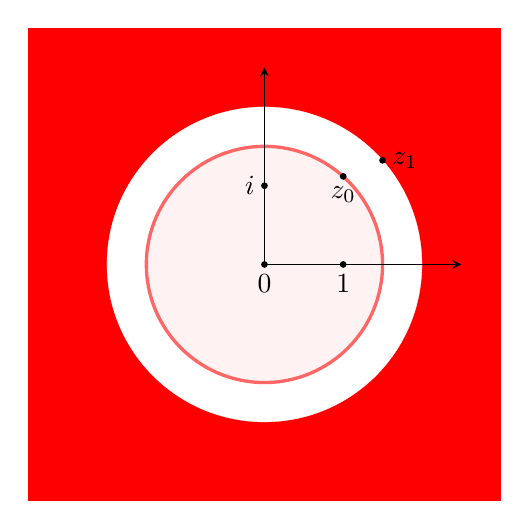
\begin{tikzpicture}
\filldraw [red] (-3,-3) rectangle (3,3);
\filldraw[color=white!60, fill=white!5, ultra thin](0,0) circle (2);
\filldraw[black] (1.5,1.32287566) circle (1pt) node[anchor=west]{$z_1$};
\filldraw[color=red!60, fill=red!5, very thick](0,0) circle (1.5);
\filldraw[black] (1,1.11803399) circle (1pt) node[anchor=north]{$z_0$};
\draw [-stealth](0,0) -- (2.5,0);
\filldraw[black] (0,0) circle (1pt) node[anchor=north]{$0$};
\filldraw[black] (1,0) circle (1pt) node[anchor=north]{$1$};
\filldraw[black] (0,1) circle (1pt) node[anchor=east]{$i$};
\draw [-stealth](0,0) -- (0,2.5);
\end{tikzpicture}
\end{center}
\caption{Une petite illustration de lemme d'Abel }
\label{fig:Abel Illutrastion}
\end{figure}


Dans cette figure $z_0$ est une point de convergence de série… Il donne comme conséquence la convergence de série en tout point dans le cercle rose (c.-à-d. lorsque $|z|<|z_0|$), mais on ne peut rien dire la frontière en rouge.
\\ D'autre part : $z_1$ est une point de divergence de série... il résulte de cela que tout la en gris ne contient que des points de divergence (c.-à-d. lorsque $|z|>|z_1|$.
\\ De cela, on a déterminé la nature de série en tout point sauf le cercle blanche [et la frontière rose] … pour fixer ce problème, on cherche à "maximiser" $|z_0|$ et "minimiser" $|z_1|$ pour éliminer cette partie blanche. D'où la définition suivante : 

\defn{Définition de Rayon de Convergence}{
On définit le rayon de convergence pour la série entière : $ \sum a_nz^n \tq z\in\CC $ par : 
\[ \rcv = \sup{ \{|z| \tq z\in\CC,\sum_n a_nz^n \text{  conv} \} } \]
NB : avec les conventions. 
\begin{itemize}
	\item Si $ \{|z| \tq z\in\CC,\sum_n a_nz^n \text{  conv} \} =\emptyset $     \ \ : on convient $\rcv = 0$
	\item Si $ \{|z| \tq z\in\CC,\sum_n a_nz^n \text{  conv} \} =\RR^+ $ : on convient $\rcv = +\infty$
\end{itemize}
on peut aussi noter : $\rcv=\rcv( (a_n)_{n\in\NN } )$
}

On peut déduire la méthode suivante qui permet en plusieurs cas de déterminer le \rcv 

\meth{Détermination de \rcv}{
Soit la série entière : $ \sum a_nz^n \tq z\in\CC $ et soit $r\in\RR^+$ , pour montrer que $\rcv=r$ il suffit de vérifier ces deux conditions  :
\begin{enumerate}
\item $\forall x \in [0,r[ \text{ \ : } \sum_n a_nx^n \text{ \ conv}$ [ce qui fait ,généralement, l'appelle aux séries géométriques].
\item $\sum_n a_nr^n \text{ \ div}$  [ cette cas est fréquente dans les exercices ].
\end{enumerate}
}


\exm{}{
Mq  rayon de convergence de série entière : $\sum_n cos(n)z^n $ est égal à $1$: \\
\textbf{Solution  : } \\
soit $x \in [0,1[$ on a : $|cos(n)x^n| =O(x^n) $ et comme $|x|<1$ alors : $\sum_n x^n $ conv et par conséquence  $\sum_n cos(n)x^n $ conv.
\\ 
Pour $x = 1$ :  $\sum_n cos(n) $ div, car $(cos(n))_{n\in\NN} $ div (donc ne converge pas vers 0) … cela sera laissé exercice pour le lecteur.
}

Il y en a aussi les deux théorèmes suivants : 
\thm{Règle D'Alembert pour calculer le \rcv \label{thm:DalebertSE}}{
Soit la série entière : $ \sum a_nz^n \tq z\in\CC $ tq [APCR] la suite $(a_n)_{n\in\NN } $ ne s'annule pas, et si on pose [ sous la condition d'existence ] $\displaystyle  l=\lim_{n \to +\infty} \frac{a_{n+1}}{a_n} $.
\\ Sous ces deux conditions [ ne s'annule pas, existence de limite] on a : 
\[ \rcv = \frac{1}{l} = \frac{1}{\displaystyle \lim_{n \to +\infty} \frac{a_{n+1}}{a_n}}\] 
}
\thm{Comparaison des \rcv}{ 
Soit les suites $ (a_n)_{ n \in \NN}  \text{ \ et \ }  (b_n)_{n\in\NN } $ et, soit $ a=\rcv ( (a_n)_{n\in\NN } ) $ et $ b=\rcv ( (b_n)_{n\in\NN } ) $
\\ Alors, on a  : 
\begin{itemize}
\item Si $a_n = o(b_n) $ \ \ \ \ \ \ \ \ \ \ \  alors : $ a \leq b $
\item Si $a_n = O(b_n) $ \ \ \ \ \ \ \ \ \ \  alors : $ a \leq b $
\item Si $\forall n\in\NN \two  a_n \leq b_n $ alors : $ a \leq b $
\item Si $a_n \sim b_n$ \ \ \ \ \ \ \ \ \ \ \ \ \ \ \ alors : $a=b$
\end{itemize}
}

\exm{}{
Calculer rcv des séries entières suivantes :
\begin{enumerate}
\item $\sum_n \frac{n^n}{n!}z^n$
\item $\sum_n \int_0^1 \frac{dt}{(1+t+t^2)^n}z^n $
\end{enumerate}
\textbf{\\ Solution : \\}
\begin{enumerate}
\item Il suffit là appliquer la règle d'Alembert (les conditions sont bien vérifiées, la suite ne s'annule pas ), en effet : 
\[ \frac{(n+1)^{(n+1)}}{(n+1)!}\times \frac{n!}{n^n}  \underset{n \longrightarrow +\infty}{\longrightarrow} e  \]
Et alors \rcv = e. 
\item Il suffit de remarque que : $\forall t \in [0,1]$ : $(1+t)\leq (1+t+t^2) \leq (1+2t+t^2)=(1+t)^2$ et alors : 
\[ 	 \int_0^1 \frac{dt}{(1+t)^{2n}} \leq \int_0^1 \frac{dt}{(1+t+t^2)^n} \leq \int_0^1 \frac{dt}{(1+t)^n}= \]
Or : 
\begin{itemize}
\item $ \displaystyle \int_0^1 \frac{dt}{(1+t)^{n}} = \frac{1}{n-1}\times \left( 1-\frac{1}{2^{n-1}} \right) \sim \frac{1}{n} $
\item De même : $ \displaystyle \int_0^1 \frac{dt}{(1+t)^{2n}} \sim \frac{1}{2n}  $
\end{itemize}
De plus $\rcv \left( \displaystyle \sum_n \int_0^1 \frac{dt}{(1+t)^{n}} z^n  \right) = \rcv \left( \displaystyle \sum_n \int_0^1 \frac{dt}{(1+t)^{2n}} z^n \right) = 1$ et comme : \[\rcv \left( \displaystyle \sum_n \int_0^1 \frac{dt}{(1+t)^{2n}} z^n  \right) \leq \rcv \left( \displaystyle \sum_n \int_0^1 \frac{dt}{(1+t+t^2)^{n}} z^n  \right)  \leq \rcv \left( \displaystyle \sum_n \int_0^1 \frac{dt}{(1+t)^{n}} z^n  \right) \]
Ce qui donne : $ \rcv \left( \displaystyle \sum_n \int_0^1 \frac{dt}{(1+t+t^2)^{n}} z^n  \right) = 1 $
\end{enumerate}
}


\newpage
\section{Exercices  }

\exop{Développement asymptotique de série Harmonique | extrait CNC'2021 }{
Pour tout entier naturel non nul $n$, on pose $H_{n}=\displaystyle%
\sum\limits_{k=1}^{n}\displaystyle\frac{1}{k}$ et $u_{n}=H_{n}-\ln (n)$,
\begin{enumerate}
\item
\begin{enumerate}
\item Justifier que la suite $\left( u_{n}\right) _{n\geq _{1}}$ converge.
On note $\gamma $ ta limite.

\item Montrer que pour tout entier $n$ tel que $n\geq 2,\ \displaystyle%
\sum\limits_{k=2}^{n}\displaystyle\frac{1}{k}\leq \ln n\leq \displaystyle%
\sum\limits_{k=1}^{n-1}\displaystyle\frac{1}{k}$

\item En déduire que $0\leq \gamma \leq 1$. \newline
\end{enumerate}

\item On pose pour tout entier naturel non nul $n,\ v_{n}=u_{n}-\gamma $.

\begin{enumerate}
\item Vérifier que $\gamma =1+\displaystyle\sum\limits_{n=2}^{+\infty
}\left( \displaystyle\frac{1}{n}-\ln \left( \displaystyle\frac{n}{n-1}%
\right) \right) $.

\item En déduire que $v_{n}=\displaystyle\sum\limits_{k=n+1}^{+\infty
}\left( \ln \left( \displaystyle\frac{k}{k-1}\right) -\displaystyle\frac{1}{k%
}\right) $.

\item Conclure que $H_{n}=\ln (n)+\gamma +\displaystyle\frac{1}{2n}+o\left( %
\displaystyle\frac{1}{n}\right) $. \newline
\end{enumerate}

\item On pose pour tout entier naturel non nul $n$; $\ w_{n}=u_{n}-\gamma -%
\displaystyle\frac{1}{2n}$.

\begin{enumerate}
\item Donner un équivalent simple de $w_{n+1}-w_{n}$.

\item Trouver un équivalence simple de :  
$\displaystyle\sum\limits_{k=n}^{+\infty }\displaystyle\frac{1}{%
k^{3}}$

\item Conclure que $H_{n}=\ln (n)+\gamma +\displaystyle\frac{1}{2n}-\displaystyle\frac{1}{12n^{2}}+o\left( \displaystyle\frac{1}{n^{2}}\right) $.
\newline
\end{enumerate}
\end{enumerate}
}{
\begin{enumerate}
\item
\begin{enumerate}
\item On a
\begin{eqnarray*}
u_{n}-u_{n+1} &=&H_{n}-\ln (n)-H_{n+1}+\ln (n+1) \\
&=&\ln (1+\frac{1}{n})-\frac{1}{n+1}
\end{eqnarray*}%
De plus
\begin{equation*}
\ln (1+\frac{1}{n})=\frac{1}{n}-\frac{1}{2n^{2}}+o(\frac{1}{n^{2}})
\end{equation*}
et
\begin{equation*}
\frac{1}{n+1}=\frac{1}{n}\frac{1}{1+\frac{1}{n}}=\frac{1}{n}-\frac{1}{n^{2}}%
+o(\frac{1}{n^{2}})
\end{equation*}

Par suite $u_{n}-u_{n+1}=\displaystyle\frac{1}{2n^{2}}+o(\displaystyle\frac{1%
}{n^{2}})$ et \fbox{$\left( u_{n}-u_{n+1}\right) \underset{n\rightarrow
+\infty }{\sim }\displaystyle\frac{1}{2n^{2}}$} .

 Comme $\left( u_{n}-u_{n+1}\right) \underset{n\rightarrow +\infty }{%
\sim }\displaystyle\frac{1}{2n^{2}}$ alors $\left( u_{n}-u_{n+1}\right) $
est positive \`{a} partir d'un certain rang , la s\'{e}rie $%
\sum\limits_{n\geq 1}\frac{1}{n^{2}}$ converge , par comparaison la s\'{e}%
rie $\sum\limits_{n\geq 1}\left( u_{n}-u_{n+1}\right) $ converge .
 Soit $S_{n}$ la somme partielle de la s\'{e}rie $\sum\limits_{n\geq
1}\left( u_{n}-u_{n+1}\right) $ . On a
\begin{equation*}
S_{n}=\sum\limits_{k=1}^{n}\left( u_{k}-u_{k+1}\right) =u_{1}-u_{n+1}
\end{equation*}
donc $u_{n}=u_{1}-S_{n-1}$ . La convergence de $\sum\limits_{n\geq 1}\left(
u_{n}-u_{n+1}\right) $ entraine la convergence de $\left( S_{n}\right)
_{n\geq 1}$et de la suite $\left( u_{n}\right) _{n\geq 1}$.

\item Soit $n\geq 2,$et $1\leq k\ \leq n-1$ . Pour $t\in \left[ k,k+1\right]
\ $on a $\displaystyle\frac{1}{k+1}\leq \displaystyle\frac{1}{t}\leq %
\displaystyle\frac{1}{k}$ ce qui donne
\begin{equation*}
\fbox{$\displaystyle\frac{1}{k+1}\leq \displaystyle\int_{k}^{k+1}%
\displaystyle\frac{dt}{t}\leq \displaystyle\frac{1}{k}$}.
\end{equation*}%
\newline
Donc $\ $%
\begin{equation*}
\displaystyle\sum\limits_{k=1}^{n-1}\frac{1}{k+1}\leq \displaystyle%
\int_{1}^{n}\displaystyle\frac{dt}{t}\leq \displaystyle\sum%
\limits_{k=1}^{n-1}\displaystyle\frac{1}{k}
\end{equation*}
ainsi
\begin{equation*}
\fbox{$\displaystyle\sum\limits_{k=2}^{n}\displaystyle\frac{1}{k}\leq \ln
n\leq \displaystyle\sum\limits_{k=1}^{n-1}\displaystyle\frac{1}{k}$}
\end{equation*}

\item D'apr\`{e}s d) $H_{n}-1\leq \ln n\leq H_{n}-\frac{1}{n},\ $donc $\frac{%
1}{n}\leq H_{n}-\ln (n)\leq 1\ ,\ $par passage \`{a} la limite on obtient
\fbox{$0\leq \gamma \leq 1$}.
\end{enumerate}
\item
\begin{enumerate}
\item D'apr\`{e}s c) on a $u_{n}=u_{1}-S_{n-1}$ et $u_{1}=1\ $de plus $%
u_{n}-u_{n+1}=\ln \left( \displaystyle\frac{n+1}{n}\right) -\displaystyle%
\frac{1}{n+1}$ , donc
\begin{eqnarray*}
u_{n} &=&1-\sum\limits_{k=1}^{n-1}\ln (1+\frac{1}{k})-\frac{1}{k+1} \\
&=&1+\sum\limits_{k=2}^{n}\frac{1}{k}-\ln (\frac{k}{k-1})
\end{eqnarray*}%
\newline
Par passage à la limite on obtient \cc{\gamma =1+\displaystyle%
\sum\limits_{n=2}^{+\infty }\left( \displaystyle\frac{1}{n}-\ln \left( %
\displaystyle\frac{n}{n-1}\right) \right) }.

\item On a : $$v_{n}=u_{n}-\gamma =\sum\limits_{k=2}^{n}\frac{1}{k}-\ln (\frac{k}{k-1%
})-\sum\limits_{k=2}^{+\infty }\frac{1}{k}-\ln (\frac{k}{k-1})$$ donc :  $$\displaystyle v_{n}=\sum\limits_{k=n+1}^{+\infty }\left( \ln \left( 
\frac{k}{k-1}\right) -\frac{1}{k}\right)$$ C'est
le reste de la série $$\sum\limits_{k\geq 2}\left( \ln \left( \frac{k}{k-1%
}\right) -\frac{1}{k}\right) $$

\item On a
\begin{eqnarray*}
\ln \left( \frac{k}{k-1}\right) -\frac{1}{k} &=&-\ln \left( 1-\frac{1}{k}%
\right) -\frac{1}{k} \\
&=&\frac{1}{2k^{2}}+o(\frac{1}{k^{2}})
\end{eqnarray*}%
donc $\ln \left( \frac{k}{k-1}\right) -\frac{1}{k}\underset{n\rightarrow
+\infty }{\sim }\frac{1}{2k^{2}}$ , les deux s\'{e}ries $\sum \ln \left(
\frac{k}{k-1}\right) -\frac{1}{k}$ et $\sum \frac{1}{2k^{2}}$ convergents,
donc les restes sont équivalents, ce qui donne $v_{n}\underset{%
n\rightarrow +\infty }{\sim }\displaystyle\sum\limits_{k=n+1}^{+\infty }%
\displaystyle\frac{1}{2k^{2}}$, ainsi
\begin{equation*}
v_{n}\underset{n\rightarrow +\infty }{\sim }\displaystyle\frac{1}{2n}
\end{equation*}%
car si $\alpha >1\ $alors $\sum\limits_{k=n+1}^{+\infty }\frac{1}{k^{\alpha }%
}\underset{n\rightarrow +\infty }{\sim }\frac{1}{(\alpha -1)n^{\alpha -1}}$ $%
.$\newline
On a $v_{n}=\frac{1}{2n}+o(\frac{1}{n})$ donc : \cc{H_{n}=\ln (n)+\gamma
+v_{n}=\ln (n)+\gamma +\frac{1}{2n}+o\left( \frac{1}{n}\right) } \newline
\end{enumerate}

\item On pose pour tout entier naturel non nul $n$; $\ w_{n}=u_{n}-\gamma -%
\frac{1}{2n}$.

\begin{enumerate}
\item On a
\begin{equation*}
w_{n+1}-w_{n}=u_{n+1}-u_{n}+\frac{1}{2n}-\frac{1}{2(n+1)}
\end{equation*}
et
\begin{equation*}
u_{n}-u_{n+1}=\ln (1+\frac{1}{n})-\frac{1}{n+1}
\end{equation*}
donc$\ $%
\begin{equation*}
w_{n+1}-w_{n}=-\ln (1+\frac{1}{n})+\frac{1}{2(n+1)}+\frac{1}{2n}.
\end{equation*}
Comme
\begin{equation*}
\ln (1+\frac{1}{n})=\frac{1}{n}-\frac{1}{2n^{2}}+\frac{1}{3n^{3}}+o(\frac{1}{%
n^{3}})
\end{equation*}%
et
\begin{eqnarray*}
\frac{1}{n+1} &=&\frac{1}{n}\times \left(\frac{1}{1+\frac{1}{n}}\right)  \\
&=&\frac{1}{n}-\frac{1}{n^{2}}+\frac{1}{n^{3}}+o(\frac{1}{n^{3}})
\end{eqnarray*}%
alors%
\begin{eqnarray*}
w_{n+1}-w_{n} &=&\left( -\frac{1}{n}+\frac{1}{2n^{2}}-\frac{1}{3n^{3}}
\right) +\left( \frac{1}{n}-\frac{1}{2n^{2}}+\frac{1}{2n^{3}}\right) +o(
\frac{1}{n^{3}}) \\
&=&\frac{1}{6n^{3}}+o(\frac{1}{n^{3}})
\end{eqnarray*}
et $$w_{n+1}-w_{n} \underset{n\rightarrow +\infty }{\sim }
\displaystyle\frac{1}{6n^{3}}$$

\item On a
\begin{eqnarray*}
\frac{1}{n^{2}}-\frac{1}{(n+1)^{2}} &=&\frac{1}{n^{2}}\left( 1-\left( 1+%
\frac{1}{n}\right) ^{-2}\right) \\
&=&\frac{1}{n^{2}}\left( 1-\left( 1-\frac{2}{n}+o(\frac{1}{n})\right) \right)
\\
&=&\frac{2}{n^{3}}+o(\frac{1}{n^{3}})
\end{eqnarray*}%
donc
\begin{equation*}
\frac{1}{n^{2}}-\frac{1}{(n+1)^{2}}\underset{n\rightarrow +\infty }{\sim }%
\frac{2}{n^{3}}
\end{equation*}
les deux s\'{e}ries$\ \sum $ $\frac{1}{n^{2}}-\frac{1}{(n+1)^{2}},\sum \frac{%
2}{n^{3}}$ convergent donc les restes sont \'{e}quivalents , de plus
\begin{eqnarray*}
\sum\limits_{k=n+1}^{+\infty }\left( \frac{1}{k^{2}}-\frac{1}{(k+1)^{2}}%
\right) &=&\lim\limits_{N\rightarrow +\infty }\sum\limits_{k=n+1}^{N}\left(
\frac{1}{k^{2}}-\frac{1}{(k+1)^{2}}\right) \\
&=&\lim\limits_{N\rightarrow +\infty }\left( \frac{1}{(n+1)^{2}}-\frac{1}{%
(N+1)^{2}}\right) \\
&=&\frac{1}{(n+1)^{2}}
\end{eqnarray*}%
Ainsi
\begin{equation*}
\fbox{$\displaystyle\sum\limits_{k=n}^{+\infty }\displaystyle\frac{1}{k^{3}}%
\underset{n\rightarrow +\infty }{\sim }\displaystyle\frac{1}{2n^{2}}$}
\end{equation*}

\item On a pour tout entier naturel non nul$\mathrm{\ }n$,
\begin{equation*}
w_{n}=u_{n}-\gamma -\frac{1}{2n}\ \text{et }w_{n+1}-w_{n}\underset{%
n\rightarrow +\infty }{\sim }\frac{1}{6n^{3}}
\end{equation*}%
donc la s\'{e}rie $\sum \left( w_{n+1}-w_{n}\right) $ converge. \newline
Remarquons que la somme partielle $\displaystyle\sum\limits_{k=1}^{n-1}%
\left( w_{k+1}-w_{k}\right) =w_{n}-w_{1}$ et $w_{n}\underset{n\rightarrow
+\infty }{\rightarrow }0$ donc%
\begin{equation*}
\sum\limits_{k=1}^{+\infty }\left( w_{k+1}-w_{k}\right) =-w_{1}
\end{equation*}%
et le reste
\begin{equation*}
\sum\limits_{k=n}^{+\infty }\left( w_{k+1}-w_{k}\right) \underset{%
n\rightarrow +\infty }{\sim }\frac{1}{6}\sum\limits_{k=n}^{+\infty }\frac{1}{%
k^{3}}
\end{equation*}%
donc
\begin{equation*}
\sum\limits_{k=n}^{+\infty }\left( w_{k+1}-w_{k}\right) =\frac{1}{12n^{2}}+o(%
\frac{1}{n^{2}}).
\end{equation*}%
\newline
Des relations
\begin{eqnarray*}
\sum\limits_{k=1}^{+\infty }\left( w_{k+1}-w_{k}\right) &=&-w_{1} \\
&=&\sum\limits_{k=1}^{n-1}\left( w_{k+1}-w_{k}\right)
+\sum\limits_{k=n}^{+\infty }\left( w_{k+1}-w_{k}\right) \\
&=&w_{n}-w_{1}+\frac{1}{12n^{2}}+o(\frac{1}{n^{2}}).
\end{eqnarray*}%
\newline
on a
\begin{equation*}
w_{n}=\frac{-1}{12n^{2}}+o(\frac{1}{n^{2}}).
\end{equation*}%
\newline
Comme $H_{n}=w_{n}+\ln (n)+\gamma +\frac{1}{2n}\ $alors
\begin{equation*}
\fbox{$H_{n}=\ln (n)+\gamma +\frac{1}{2n}-\frac{1}{12n^{2}}+o\left( \frac{1}{%
n^{2}}\right) $}
\end{equation*}%
\newline
\end{enumerate}
\end{enumerate}
}


\end{document}






